\documentclass[11pt]{article}
% Portable XeLaTeX preprint style. Fonts are looked up by TeX Live filenames.
\usepackage{fontspec}
\setmainfont{texgyretermes-regular.otf}[BoldFont=texgyretermes-bold.otf,ItalicFont=texgyretermes-italic.otf,BoldItalicFont=texgyretermes-bolditalic.otf]
\setsansfont{texgyreheros-regular.otf}[BoldFont=texgyreheros-bold.otf,ItalicFont=texgyreheros-italic.otf,BoldItalicFont=texgyreheros-bolditalic.otf,Scale=MatchLowercase]
\setmonofont{lmmono10-regular.otf}[Scale=MatchLowercase]
\usepackage{amsmath,amsthm}
\usepackage{unicode-math}
\setmathfont{texgyretermes-math.otf}
\usepackage[a4paper,top=23mm,bottom=23mm,left=24mm,right=24mm,headheight=14pt,headsep=8mm,footskip=12mm]{geometry}
\usepackage{graphicx,booktabs,caption,needspace,placeins,xcolor}
\definecolor{Ink}{HTML}{183447}
\definecolor{Accent}{HTML}{126B78}
\definecolor{Muted}{HTML}{53626C}
\usepackage{titlesec}
\titleformat{\section}{\normalfont\bfseries\large\color{Ink}}{\thesection}{0.65em}{}
\titleformat{\subsection}{\normalfont\bfseries\color{Ink}}{\thesubsection}{0.65em}{}
\titlespacing*{\section}{0pt}{17pt plus 2pt minus 2pt}{8pt}
\titlespacing*{\subsection}{0pt}{12pt plus 2pt minus 1pt}{6pt}
\usepackage{fancyhdr}
\pagestyle{fancy}
\fancyhf{}
\fancyhead[L]{\small\color{Muted}Packing 68 unit squares in a circle}
\fancyhead[R]{\small\color{Muted}ShaneZhang}
\fancyfoot[C]{\small\thepage}
\renewcommand{\headrulewidth}{0.25pt}
\renewcommand{\footrulewidth}{0pt}
\usepackage[colorlinks=true,linkcolor=Accent,citecolor=Accent,urlcolor=Accent,unicode]{hyperref}
\usepackage{url}
\urlstyle{same}
\captionsetup{font=small,labelfont={bf,color=Ink},labelsep=period,skip=7pt,justification=justified,singlelinecheck=false}
\setlength{\parindent}{1em}
\setlength{\parskip}{1.5pt plus 0.3pt}
\linespread{1.045}
\setlength{\textfloatsep}{15pt plus 2pt minus 2pt}
\setlength{\intextsep}{13pt plus 2pt minus 2pt}
\setlength{\floatsep}{12pt}
\renewcommand{\topfraction}{0.92}
\renewcommand{\bottomfraction}{0.8}
\renewcommand{\textfraction}{0.06}
\renewcommand{\floatpagefraction}{0.75}
\setcounter{topnumber}{2}
\emergencystretch=1.6em
\widowpenalty=10000
\clubpenalty=10000
\displaywidowpenalty=10000
\brokenpenalty=10000
\raggedbottom
\newcommand{\R}{\mathbb R}
\newcommand{\Q}{\mathbb Q}
\newcommand{\disk}{D}
\newcommand{\area}{\operatorname{area}}
\newcommand{\suppfile}[1]{\path{#1}}
\newtheoremstyle{paperthm}{8pt}{8pt}{\normalfont}{}{\bfseries\color{Ink}}{.}{0.5em}{}
\theoremstyle{paperthm}

\newtheorem{theorem}{Theorem}
\newtheorem{lemma}{Lemma}
\newtheorem{proposition}{Proposition}
\hypersetup{pdftitle={Strict bounds for packing 68 unit squares in a circle},pdfauthor={ShaneZhang},pdfsubject={An exact construction and a computer-assisted lower bound}}
\begin{document}
\thispagestyle{plain}
\begin{center}
{\small\sffamily\color{Muted} PREPRINT\quad |\quad 30 OCTOBER 2026\par}
\vspace{13pt}
{\fontsize{22}{25}\selectfont\bfseries\color{Ink}
Strict bounds for packing\\[2pt]
68 unit squares in a circle\par}
\vspace{14pt}
{\large ShaneZhang\par}
\vspace{4pt}
Shanghai University\\[2pt]
\href{mailto:chromoany@Gmail.com}{\small chromoany@Gmail.com}
\end{center}
\vspace{10pt}
\begin{abstract}

Let $r(68)$ be the infimum of radii of disks containing 68 unit squares with arbitrary orientations and pairwise disjoint interiors. We give a rational-coordinate construction and a computer-assisted exclusion proving
\[
\frac{39}{8}<r(68)<5.031404629453352.
\]
The construction has an exact enclosing radius specified by a quadratic equation with integer coefficients and an isolating interval of width $10^{-30}$. The lower bound uses a nonnegative radial weight on 80 annuli. Its single-square inequality is verified on a complete subdivision of a continuous two-dimensional domain, using exact rational arithmetic and outward interval bounds. Coordinates, weights, subdivision data and verification programs accompany the paper. The exact optimum and feasibility at radius $5$ remain open.

\end{abstract}
\smallskip
\noindent{\small\textbf{Keywords.} Square packing; disk; exact construction; weighted area; computer-assisted proof.}

\section{Introduction and main result}
Write $D_R=\{z\in\R^2:\|z\|\le R\}$. A packing consists of closed unit squares whose interiors are pairwise disjoint; tangency is permitted. Translations and rotations of the squares are unrestricted. Translating the enclosing disk to the origin does not restrict the problem. We define $r(68)$ as the infimum of feasible radii.

\begin{theorem}\label{thm:main}
There is an explicitly specified packing of 68 unit squares with rational centers and rational unit direction vectors. If $\widehat R$ is its enclosing radius about the specified origin, then
\begin{equation}\label{eq:bounds}
\frac{39}{8}<r(68)\le\widehat R<U,
\qquad U=\frac{5031404629453352}{10^{15}}.
\end{equation}
Moreover,
\begin{equation}\label{eq:isolation}
\begin{gathered}
5.031404629453350730787899409097
<\widehat R,\\
\widehat R<5.031404629453350730787899409098.
\end{gathered}
\end{equation}
\end{theorem}

Montanher et al.~\cite{montanher} study the same freely rotating square-in-circle problem and give rigorous interval enclosures for the three-square optimum and its configurations. The distinction between approximate feasibility and proved feasibility is also central to Domes and Neumaier~\cite{domes}. For a direct historical comparison at $n=68$, Jelliss~\cite{jelliss} describes a grid construction of radius $\sqrt{26}$. The upper bound in \eqref{eq:bounds} is smaller, since $U^2<26$. This comparison does not assert a current record or priority over all published constructions.

The elementary area bound is $r(68)\ge\sqrt{68/\pi}\approx4.65242649$; the present strict lower bound raises this baseline to $39/8=4.875$. Our contribution is an explicit exact construction together with a reproducible exclusion certificate over all real poses. Friedman's collection~\cite{friedman} provides further context for smaller instances; the version consulted lists $n\le50$ and supplies no comparison at $n=68$.

The lower-bound method assigns a minimum weighted area to every admissible square. Resource-counting arguments of this kind have predecessors in the unavoidable-set method of Kearney and Shiu~\cite{kearney}. A recent preprint of Karakuş~\cite{karakus} discusses more general nonnegative measures for packing bounds. Here the counting inequality itself is elementary; the substantive certificate verifies a particular radial weight for every real translation and orientation in a disk. Section~\ref{sec:validation} explains why its finite computations cover this continuous family.

\section{An exact upper-bound certificate}\label{sec:upper}
\subsection{Rational data and geometric verification}
For each square, the data specify a center $c_i\in\Q^2$ and a vector $u_i\in\Q^2$ with $u_i\cdot u_i=1$. Let $v_i=(-u_{i,2},u_{i,1})$. Its four vertices are
\begin{equation}\label{eq:vertices}
c_i+\frac{\varepsilon u_i+\eta v_i}{2},
\qquad \varepsilon,\eta\in\{-1,1\}.
\end{equation}
Figure~\ref{fig:packing} shows the construction. It has a largely columnar interior and several rotated groups near the boundary. The exact data, rather than the plotted coordinates, define the squares.

\begin{figure}[htbp]
\centering
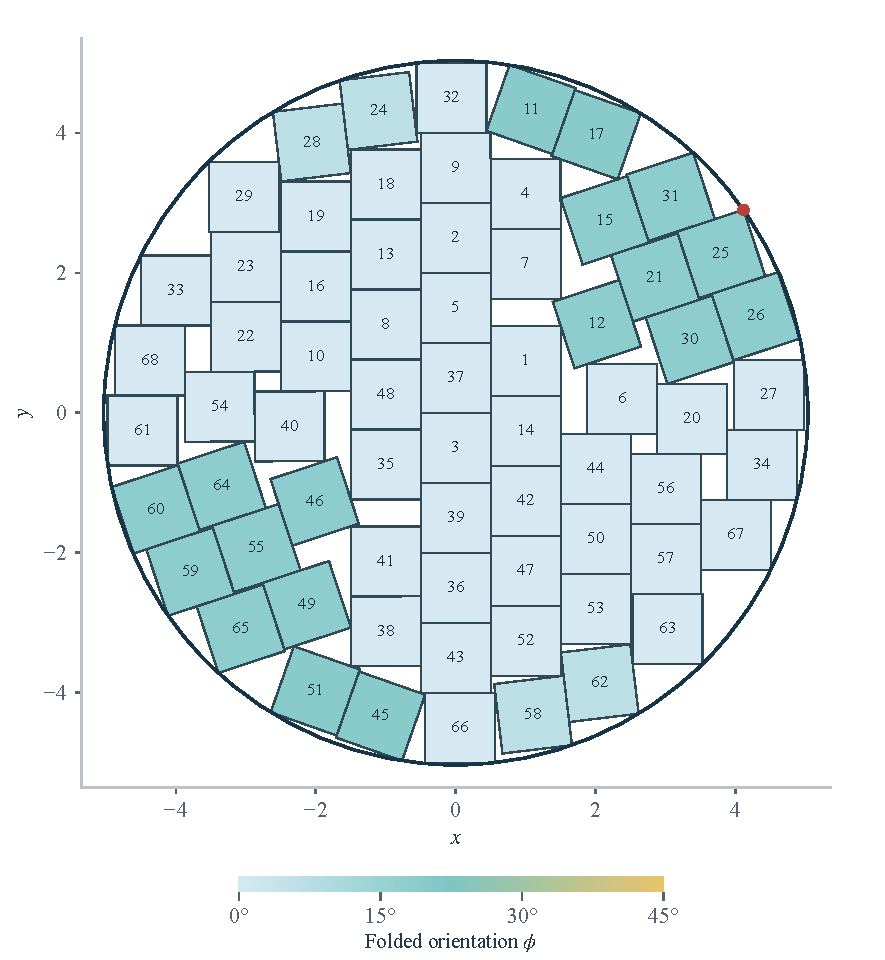
\includegraphics[width=0.89\linewidth]{figures/packing-color.pdf}
\caption{The certified 68-square construction. Labels refer to the exact coordinate file. Color records the folded orientation $\phi=\min(\alpha,90^\circ-\alpha)$, where $\alpha\in[0,90^\circ)$ is an edge angle modulo $90^\circ$. The red point is the unique farthest vertex, on square 25. All plotted coordinates are for display; the rational data define the packing.}\label{fig:packing}
\end{figure}

\Needspace{10\baselineskip}
For a pair $i<j$, put
\[
H_{ij}=\frac{1+|u_i\cdot u_j|+|\det(u_i,u_j)|}{2}.
\]
On any axis $n\in\{u_i,v_i,u_j,v_j\}$, $H_{ij}$ is the sum of the projected half-widths. Thus the squares have disjoint interiors whenever at least one such axis satisfies
\begin{equation}\label{eq:sat}
|(c_i-c_j)\cdot n|\ge H_{ij}.
\end{equation}
Conversely, the separating-axis theorem for two convex polygons shows that these four axes suffice. This can also be seen by examining the edge normals of their Minkowski difference. Equality in \eqref{eq:sat} allows boundary contact.

The accompanying verifier checks $u_i\cdot u_i=1$ for all 68 squares, \eqref{eq:sat} for all $\binom{68}{2}=2278$ pairs, and the containment of all 272 vertices. Each check is a rational comparison, hence reduces to integer arithmetic. Convexity of $D_U$ then gives containment of every square. This proves the upper-bound assertion without relying on a geometric tolerance or on the numerical search that supplied the layout.

\subsection{The exact radius of the displayed construction}
For coprime positive integers $p,q$, the exact radius is
\begin{equation}\label{eq:radius}
\widehat R=\sqrt{p/q},\qquad
\frac pq=\max_{i,\varepsilon,\eta}
\left\|c_i+\frac{\varepsilon u_i+\eta v_i}{2}\right\|^2,
\end{equation}
The maximum is attained only at square 25 with $(\varepsilon,\eta)=(1,1)$. The complete integers, of 1451 and 1450 decimal digits respectively, are supplied in \suppfile{upper/best-68-exact-radius.json}. Together with \eqref{eq:isolation}, the equation $qX^2-p=0$ specifies $\widehat R$ exactly. Squaring the rational endpoints verifies both strict inequalities in \eqref{eq:isolation} and $\widehat R<U$.

The center in this calculation is fixed. We do not assert that it is a smallest enclosing circle of this point set when the center is allowed to move. In particular, $qX^2-p$ is an equation for the displayed construction's radius, not a defining polynomial for the unknown optimum $r(68)$.

\section{A weighted-area lower bound}\label{sec:weight}
Set
\begin{equation}\label{eq:parameters}
s=\frac{40}{39},\qquad a=\frac{s}{2},\qquad
c=\frac{19926631}{20000000}.
\end{equation}
We use a nonnegative radial function $w$, constant with value $w_j\in\Q_{\ge0}$ on the annulus $j/16\le\|z\|<(j+1)/16$, for $j=0,\ldots,79$, and zero outside $D_5$. The 80 exact values are in \suppfile{lower/weights.json}; Figure~\ref{fig:weights} displays them. Values on the bounding circles have no effect on the integrals.

\begin{proposition}\label{prop:weight}
Every square $S$ of side $s$ contained in $D_5$, with arbitrary real center and orientation, satisfies
\begin{equation}\label{eq:single}
\int_S w(\|z\|)\,dz\ge c.
\end{equation}
\end{proposition}

Proposition~\ref{prop:weight} is the computer-assisted step. Its certificate and the mathematical justification of its tests are given in Section~\ref{sec:validation}.

\begin{figure}[htbp]
\centering
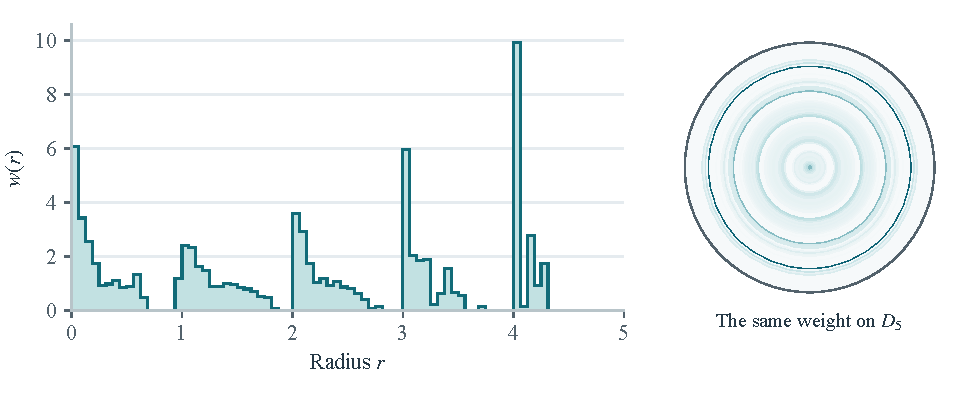
\includegraphics[width=\linewidth]{figures/weights-color.pdf}
\caption{The 80-annulus radial weight, shown as a step function (left) and on the disk $D_5$ (right). Darker annuli carry larger weight. The exact breakpoints and heights are rational, and their oscillation is retained in the signed disk-area calculation.}\label{fig:weights}
\end{figure}

\FloatBarrier
\Needspace{9\baselineskip}
The total weight is
\begin{equation}\label{eq:cost}
\begin{split}
C&=\int_{D_5}w(\|z\|)\,dz
 =\pi\sum_{j=0}^{79}w_j\frac{(j+1)^2-j^2}{256}\\
 &=\pi\frac{345050690237}{16000000000}
 <\frac{338752725}{5000000}
 <\frac{338752727}{5000000}=68c.
\end{split}
\end{equation}
For completeness, the first strict inequality needs only
\[
\pi<P:=\frac{3141592653589794}{10^{15}}.
\]
It follows from Machin's identity
$\pi=16\arctan(1/5)-4\arctan(1/239)$ and alternating-series bounds. Explicitly, if
\[
T(q,m)=\sum_{k=0}^{m}\frac{(-1)^k}{(2k+1)q^{2k+1}},
\]
then $\pi<16T(5,12)-4T(239,3)<P$; the latter comparison is rational. The gap between the last two fractions in \eqref{eq:cost} is $1/2500000$.

Suppose that 68 unit squares fit in a disk of radius at most $39/8$. Scaling the entire packing by $s=40/39$ places 68 squares of side $s$ inside $D_5$. Their interiors remain disjoint. Their boundaries have area zero, so nonnegativity and Proposition~\ref{prop:weight} imply
\[
68c\le\sum_{i=1}^{68}\int_{S_i}w
=\int_{\bigcup_i S_i}w\le C,
\]
contradicting \eqref{eq:cost}.

To obtain the strict inequality for the infimum, we also record attainment. Fix the feasible upper radius $U$. Every center in a packing inside $D_U$ has norm at most $U-1/2$, because its square contains a disk of radius $1/2$ about that center. Unit directions range over a compact circle. The vertex-containment conditions are closed, as is pairwise interior disjointness: the latter is a finite union of the closed conditions \eqref{eq:sat}. The nonempty feasible set inside $D_U$ is therefore compact. The continuous maximum of the vertex norms attains a minimum on it. Any packing that improves on $U$ belongs to this set, so this minimum is $r(68)$. The exclusion just proved yields $r(68)>39/8$ and completes Theorem~\ref{thm:main} once Proposition~\ref{prop:weight} is verified.

\Needspace{17\baselineskip}
\section{Certifying all real placements}\label{sec:validation}
The certificate is a complete binary subdivision, rather than a set of sampled placements. Its leaves carry one of three tests. We give their soundness proofs and then describe the area kernel used to evaluate them.

\subsection{Reduction and complete coverage}
For a single square, rotate it about the origin until its sides are parallel to the coordinate axes. Both its containment in $D_5$ and its radial integral are invariant. Reflections and coordinate interchange then reduce its center to $x\ge y\ge0$. This reduction is applied to the single-square integral, not separately to the squares in a packing. The admissible domain is exactly
\begin{equation}\label{eq:domain}
\Omega=\{(x,y):x\ge y\ge0,\ (x+a)^2+(y+a)^2\le25\}.
\end{equation}
The root box $B_0=[0,179/40]^2$ contains $\Omega$, since
$(179/40+a)^2+a^2>25$.
Figure~\ref{fig:cover} shows the stored subdivision and a detail of its refinement. The image is a visualization of the certificate, not a replacement for its coverage and interval checks.

\begin{figure}[htbp]
\centering
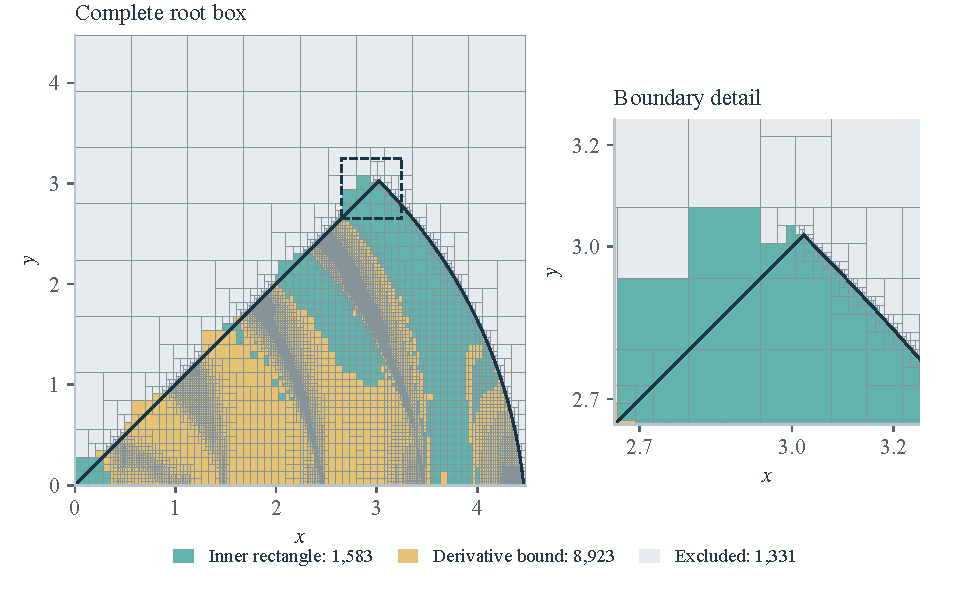
\includegraphics[width=\linewidth]{figures/cover-color.pdf}
\caption{The complete binary certificate on $B_0$, colored by leaf test, with a magnified detail on the right. The dark line marks the circular and diagonal boundaries of $\Omega$; gray boxes contain no admissible pose. The leaves are drawn directly from their stored binary paths. The exact paths and comparisons, rather than this visualization, determine coverage.}\label{fig:cover}
\end{figure}


Bisect each box through the midpoint of its longer side, choosing the $x$ direction in a tie. A binary word records a path from the root; both child boxes are closed. The supplied leaf words are distinct and prefix-free. If $d$ is their maximum length, the verifier checks the exact identity
\begin{equation}\label{eq:kraft}
\sum_{\ell\text{ a leaf}}2^{d-|\ell|}=2^d.
\end{equation}
Each word of length $d$ then has exactly one leaf prefix. All depth-$d$ boxes, and hence $B_0$, are covered, including shared boundaries.

Write a leaf box as $B=[b_0,b_1]\times[d_0,d_1]$. It contains no admissible point if
\begin{equation}\label{eq:excluded}
b_1<d_0\quad\hbox{or}\quad(b_0+a)^2+(d_0+a)^2>25.
\end{equation}
These strict rational tests do not discard a feasible boundary point.

\subsection{A common inner rectangle}
The intersection of all translated squares with centers in $B$ is
\[
K_B=[b_1-a,b_0+a]\times[d_1-a,d_0+a],
\]
provided its two side lengths are positive. Since $w\ge0$, every such square satisfies $\int_Sw\ge\int_{K_B}w$. A rigorous lower endpoint for the latter integral that is at least $c$ therefore certifies the whole box. This is the first acceptance test.

\subsection{A derivative bound}
Let $S(x,y)=[x-a,x+a]\times[y-a,y+a]$ and
\[
A_r(x,y)=\area(S(x,y)\cap D_r).
\]
With $h_r(e)=\sqrt{\max(0,r^2-e^2)}$, define the chord-intersection length
\begin{equation}\label{eq:chord}
J_r(e,z)=\max\{0,\min(z+a,h_r(e))-\max(z-a,-h_r(e))\}.
\end{equation}
This function is continuous, also at tangencies. Fubini's theorem and the fundamental theorem of calculus give
\begin{equation}\label{eq:derivative}
\begin{split}
A_r(x,y)&=\int_{x-a}^{x+a}J_r(e,y)\,de,\\
\partial_x A_r(x,y)&=J_r(x+a,y)-J_r(x-a,y).
\end{split}
\end{equation}
Interchanging $x,y$ gives the other partial derivative. Thus $A_r$ is continuously differentiable on the whole plane.

For $z\ge0$, $J_r(e,z)$ is nonincreasing in both $|e|$ and $z$: the former shrinks the centered disk chord, and the latter moves an interval of fixed length away from its center. Consequently, for $e\in[e_0,e_1]$ and $z\in[z_0,z_1]\subseteq[0,\infty)$,
\[
J_r(e_{\rm far},z_1)\le J_r(e,z)\le J_r(e_{\rm near},z_0),
\]
where $e_{\rm far}=\max(|e_0|,|e_1|)$ and $e_{\rm near}=\min_{e\in[e_0,e_1]}|e|$. Square-root enclosures and rational interval operations therefore give bounds for \eqref{eq:derivative} throughout each box.

Put $w_{80}=0$ and $r_j=j/16$. Almost everywhere,
\[
w(\|z\|)=\sum_{j=1}^{80}(w_{j-1}-w_j)\mathbf1_{D_{r_j}}(z).
\]
Hence
\begin{equation}\label{eq:integral}
I(x,y):=\int_{S(x,y)}w
=\sum_{j=1}^{80}(w_{j-1}-w_j)A_{r_j}(x,y)
\end{equation}
is continuously differentiable. Some difference coefficients are negative; interval multiplication retains their signs. If $|\partial_x I|\le M_x$ and $|\partial_y I|\le M_y$ on $B$, with midpoint $m$ and half-widths $h_x,h_y$, integration along the segment from $m$ to any point of $B$ gives
\begin{equation}\label{eq:gradient}
I(x,y)\ge\underline I(m)-M_xh_x-M_yh_y.
\end{equation}
Here $\underline I(m)$ is a rigorous lower endpoint. If the right side is at least $c$, this second acceptance test certifies every real center in the box.

\subsection{Certified disk--polygon intersection areas}
It remains to enclose the integrals in the two acceptance tests. For $r>0$ the continuous, locally Lipschitz vector field
\[
V_r(z)=\begin{cases}z/2,&\|z\|\le r,\\
r^2z/(2\|z\|^2),&\|z\|>r
\end{cases}
\]
has divergence $\mathbf1_{D_r}$ almost everywhere. For a counterclockwise polygon $P$, the divergence theorem therefore gives
\begin{equation}\label{eq:green}
\area(P\cap D_r)=\frac12\sum_{[b,b+d]\subset\partial P}
\det(b,d)\int_0^1\min\!\left(1,\frac{r^2}{\|b+td\|^2}\right)dt.
\end{equation}
The multiplier at the origin is interpreted by the continuous vector field. When $\det(b,d)=0$, the edge contributes zero.

For other edges, $q(t)=\|b+td\|^2$ is a rational quadratic. Its extrema on a rational subinterval are determined exactly by its endpoints and, if present, its vertex. A segment wholly inside the disk contributes $\det(b,d)$ times half its parameter length. A segment wholly outside contributes $r^2/2$ times the signed angle between its endpoint vectors. Because the line does not pass through the origin, this angle lies strictly between $-\pi$ and $\pi$, and the usual $\operatorname{atan2}$ branch is unambiguous.

To handle a crossing, outward square-root intervals enclose the roots of $q(t)=r^2$. Their rational endpoints, together with $0$ and $1$, subdivide the edge. A residual subinterval $[t_0,t_1]$ whose position relative to the circle remains uncertain is enclosed by the symmetric interval of radius
\[
\frac{|\det(b,d)|}{2}(t_1-t_0),
\]
because the multiplier in \eqref{eq:green} lies in $[0,1]$. Thus uncertain root locations are covered without an unproved inside/outside decision. Interval addition of the edge contributions encloses the area. Applying the signed combination in \eqref{eq:integral} encloses the weighted integral as well.

The implementation uses rational arithmetic for geometric decisions and Arb midpoint-radius intervals~\cite{johansson} at 256-bit working precision for square roots and angles. The proof depends on outward enclosure, not merely on the number of computed digits.

\subsection{The finite certificate}
The prefix test \eqref{eq:kraft} verifies 11,837 leaves, with maximum depth 24. The complete replay gives the following partition:
\begin{center}
\begin{tabular}{lr}
\toprule
Leaf test & Number\\
\midrule
Common inner rectangle & 1583\\
Derivative bound & 8923\\
Excluded by \eqref{eq:excluded} & 1331\\
\midrule
Total & 11837\\
\bottomrule
\end{tabular}
\end{center}
There are no pending leaves. Each acceptance test establishes \eqref{eq:single} throughout its box; the excluded leaves contain no point of $\Omega$. Complete coverage and rotational invariance prove Proposition~\ref{prop:weight} for all real poses.

\Needspace{17\baselineskip}
\section{Reproducibility and remaining questions}
The accompanying supplement contains the complete rational coordinates, the exact integers $p,q$, the annular weights, all leaf paths, and the verification source. In the arXiv source archive these files are in the \path{anc/} directory; the file paths cited here are relative to that directory. The upper-bound verifier uses only Python's standard-library rational arithmetic. The lower-bound replay uses \texttt{python-flint 0.8.0} and the area kernel proved above. The revised verifier uses explicit acceptance checks, rejects optimized Python execution, and has no search-resume certification entry point. A fresh complete replay verifies all 11,837 leaves; its environment and source identities are recorded in the supplement. Separate instructions explain the required final success status; a partial run is not a certificate. Source and data SHA256 digests identify the supplied files. No tolerance-dependent feasibility test is used as an acceptance criterion.

These are computer-assisted proofs, with Python and FLINT/Arb in the trusted computational base; they are not proof-assistant formalizations. The strict lower bound applies to all real placements. The exact algebraic upper radius applies to one explicit construction. The interval still contains $5$, so neither feasibility at that radius nor the exact value of $r(68)$ is decided.

\medskip
\noindent\textbf{AI assistance.} Large language models assisted proof exploration, code preparation, literature review and drafting. The accompanying programs and mathematical arguments specify the evidence supporting the claims.

\FloatBarrier
\begingroup
\raggedright
\Needspace{12\baselineskip}
\begin{thebibliography}{6}
\bibitem{montanher}
T.~Montanher, A.~Neumaier, M.~C.~Mark\'ot, F.~Domes and H.~Schichl,
Rigorous packing of unit squares into a circle,
\emph{Journal of Global Optimization} \textbf{73} (2019), 547--565.
\url{https://doi.org/10.1007/s10898-018-0711-5}.

\bibitem{domes}
F.~Domes and A.~Neumaier,
Rigorous verification of feasibility,
\emph{Journal of Global Optimization} \textbf{61} (2015), 255--278.
\url{https://doi.org/10.1007/s10898-014-0158-2}.

\bibitem{jelliss}
G.~P.~Jelliss,
Circling the squares,
\emph{The Games and Puzzles Journal}, no.~29 (2003), sections 51--55.
\url{https://mayhematics.com/j/gpj29.htm}
(accessed 30 October 2026).

\bibitem{kearney}
M.~J.~Kearney and P.~Shiu,
Efficient packing of unit squares in a square,
\emph{Electronic Journal of Combinatorics} \textbf{9}(1) (2002), Research Paper~14.
\url{https://doi.org/10.37236/1631}.

\bibitem{karakus}
H.~Karaku\c{s},
A counterexample to Nagamochi's scoring lemma and a new rectangle packing bound,
arXiv:2609.37410v1 [math.CO] (2026), preprint.
\url{https://arxiv.org/abs/2609.37410v1}.

\bibitem{johansson}
F.~Johansson,
Arb: Efficient arbitrary-precision midpoint-radius interval arithmetic,
arXiv:1611.02831v1 [cs.MS] (2016), preprint.
\url{https://arxiv.org/abs/1611.02831v1}.
\end{thebibliography}

\endgroup
\end{document}
